%\documentclass[a4paper,12pt,oneside,draft]{article}
\documentclass[a4paper,12pt,oneside]{article}

% In the original writelatex tamplate
\usepackage[english]{babel}
\usepackage[utf8]{inputenc}
\usepackage{amsmath}
\usepackage{graphicx}
\usepackage[colorinlistoftodos]{todonotes}

% By LoCigno
\usepackage{times}
\usepackage{graphicx}
\usepackage{subfigure}
\usepackage{csvsimple}
\usepackage{color}
\usepackage{url}
\usepackage{hyperref} 
\usepackage{cleveref}

% By Davide
\usepackage{comment}
\usepackage{booktabs}
\usepackage{color}

%Variables macros
\newcommand{\DefineVar}[2]{%
  \expandafter\newcommand\csname var-#1\endcsname{#2}%
} 
\newcommand{\var}[1]{\csname var-#1\endcsname}

\usepackage{courier}
\newcommand{\mono}[1]{\texttt{#1}}
%\newcommand{\mono}[1]{\texttt{\textbf{#1}}}

\title{Sentence compressor}

\author{Aliaksandr Siarohin}

\date{\today}

\begin{document}
%\maketitle
\makeatletter  % populates \@title, \@author, \@date
\begin{titlepage}
      \centering
      ~~~~~~~~~~~~~\\[-30mm]
      
\includegraphics[keepaspectratio=true, width=7cm]{bg_eng_1r.jpg} \\[10mm]

     {
     \large \bfseries Master Degree in Computer Science\\[3mm] 
     Natural Language Processing\\[3mm]
     AA 2015-2016
     }\\[10mm]

     %--------------------------------
     % Set the title, author, and date
     % 

     \vspace{0.5cm}
     {
     \Large \bfseries \textcolor{blue}{\@title} \par
     }
     \vspace{0.5cm}
%      {
%      \large {Group N. 1} \par
%      }
     \vspace{0.2cm}

     {\large {\@author}}
     \\ \vspace{.2cm}
     \@date

     \vspace{0.6cm}

    %-----------------------------------

\begin{abstract}

\textit{
  This is a description of project on natural language processing.
}


\end{abstract}

\end{titlepage}



\section {Introduction to the designed system}
In this project I implement an neural network solution to deletion-based sentence compression where the task is to translate a sentence into a sequence of zeros and ones, corresponding to token deletion decisions.

\section {The analytical model}

\subsection{Pre-processing}
The data was initially in json format. To parse json I use script provided by teaching assistant. After parsing the data become the list of list with tokens. Each token is tuple with 3 field (word, tag, stem, token deletion decision). I populate this tuple with additional field word embedding. This embedding is taken from google-news word2vec \url{https://code.google.com/archive/p/word2vec/}.

\subsection{Formal description of neural network architecture}
I use LSTM based network for this problem. The input to my network is word embedding and one hot encoding of word tag. Then there is 2 LSTM layers one which traverse the sentence from the beginning and the other which traverse it from the end. The output of this layer go to dropout layer, and the output of dropout go to the same 2 LSTM layers. Then there is dense layer with dropout. And finally dense layer with softmax non-linearity. The network structure can be found in \cref{fig:network}.

\begin{figure}[t]%
	\centering
	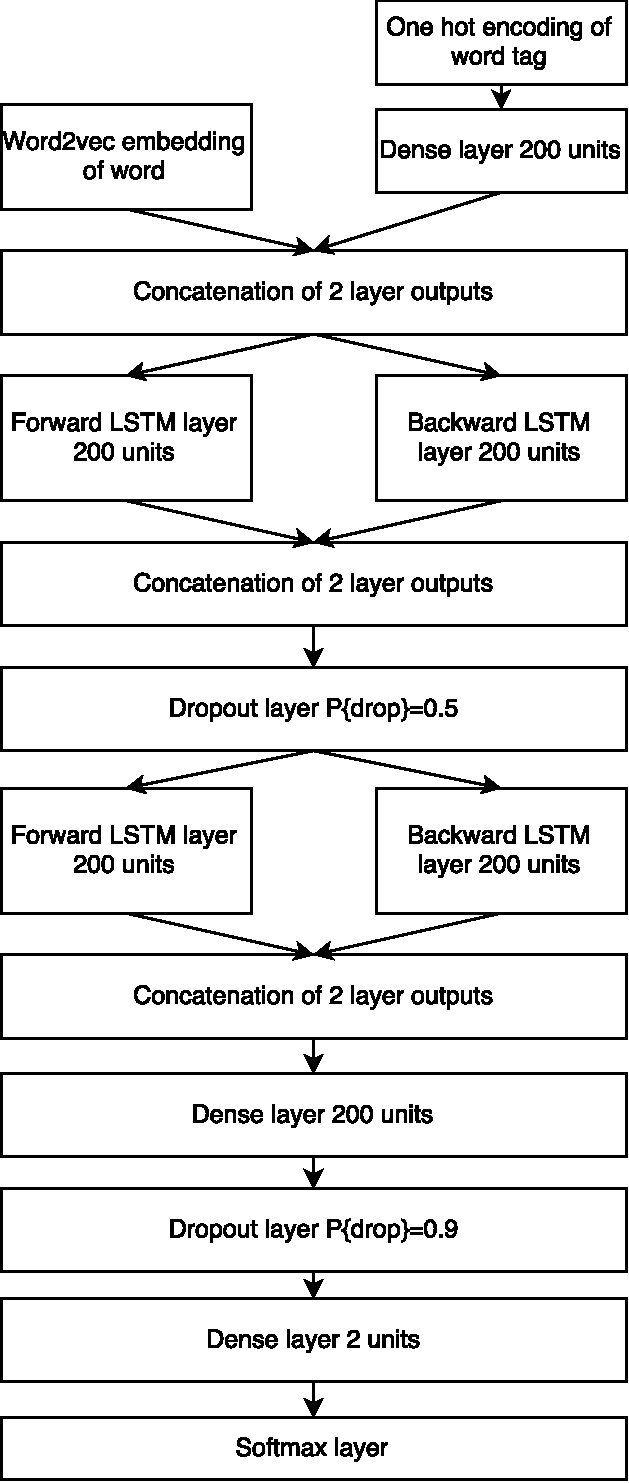
\includegraphics[width=230pt]{compression_network}
	\caption{The network architecture}%
	\label{fig:network}%
\end{figure}


\section{Software description}
To implement this project I use python library's theano+lasagne. This framework can build a graph of execution, and then evaluate it on gpu.

\subsection{Used Functions}
I use different network layers from lasagne library (LSTMLayer, DropoutLayer, DenseLayer ...). For fitting network I use adam function from lasagne library.

\section{Experiment Description}

\subsection{Data}
Data is 10000 sentences. For each word in sentence there is stem form of this word and tag of this word. Each word has associated token deletion decisions (0 or 1). For the experiment I split the data in 3 sets: train, dev and test. Test set is 1000 first sentences, train and dev set is random split of the rest 9000 sentences, 1000 for dev and 8000 for train.


\subsection{Training process}
The network is trained using adam method. The batch in my case was 1 sentence. The sentences are feed to network in random order. The training process takes 4 epochs. After each 1000 sentences I compute score for dev set and save network parameters. The network with the best score on validation set will be result. 

\subsection{Network parameters}
The size of word embedding is 300 (Because in google-news dataset it 300). The number of units in LSTM layer is 200, as well as in tag embedding. The size of last dense layer is also 200. Last layer give us probability, so in order to get 0, 1 predictions we need some threshold. In my case this threshold maximizing the f1 score on dev set and it equal to 0.505582.

\section{Result presentation}
The result score on the test set:

\begin{itemize}
  \item Per token accuracy: 0.832198
  \item Per token f1 score: 0.774660
  \item Fraction of right compression 0.162000
\end{itemize}

The learning curves can be found in \cref{fig:lcur}. The Precision/Recall curve can be found in \cref{fig:pr}.

\begin{figure}[t]%
	\centering
	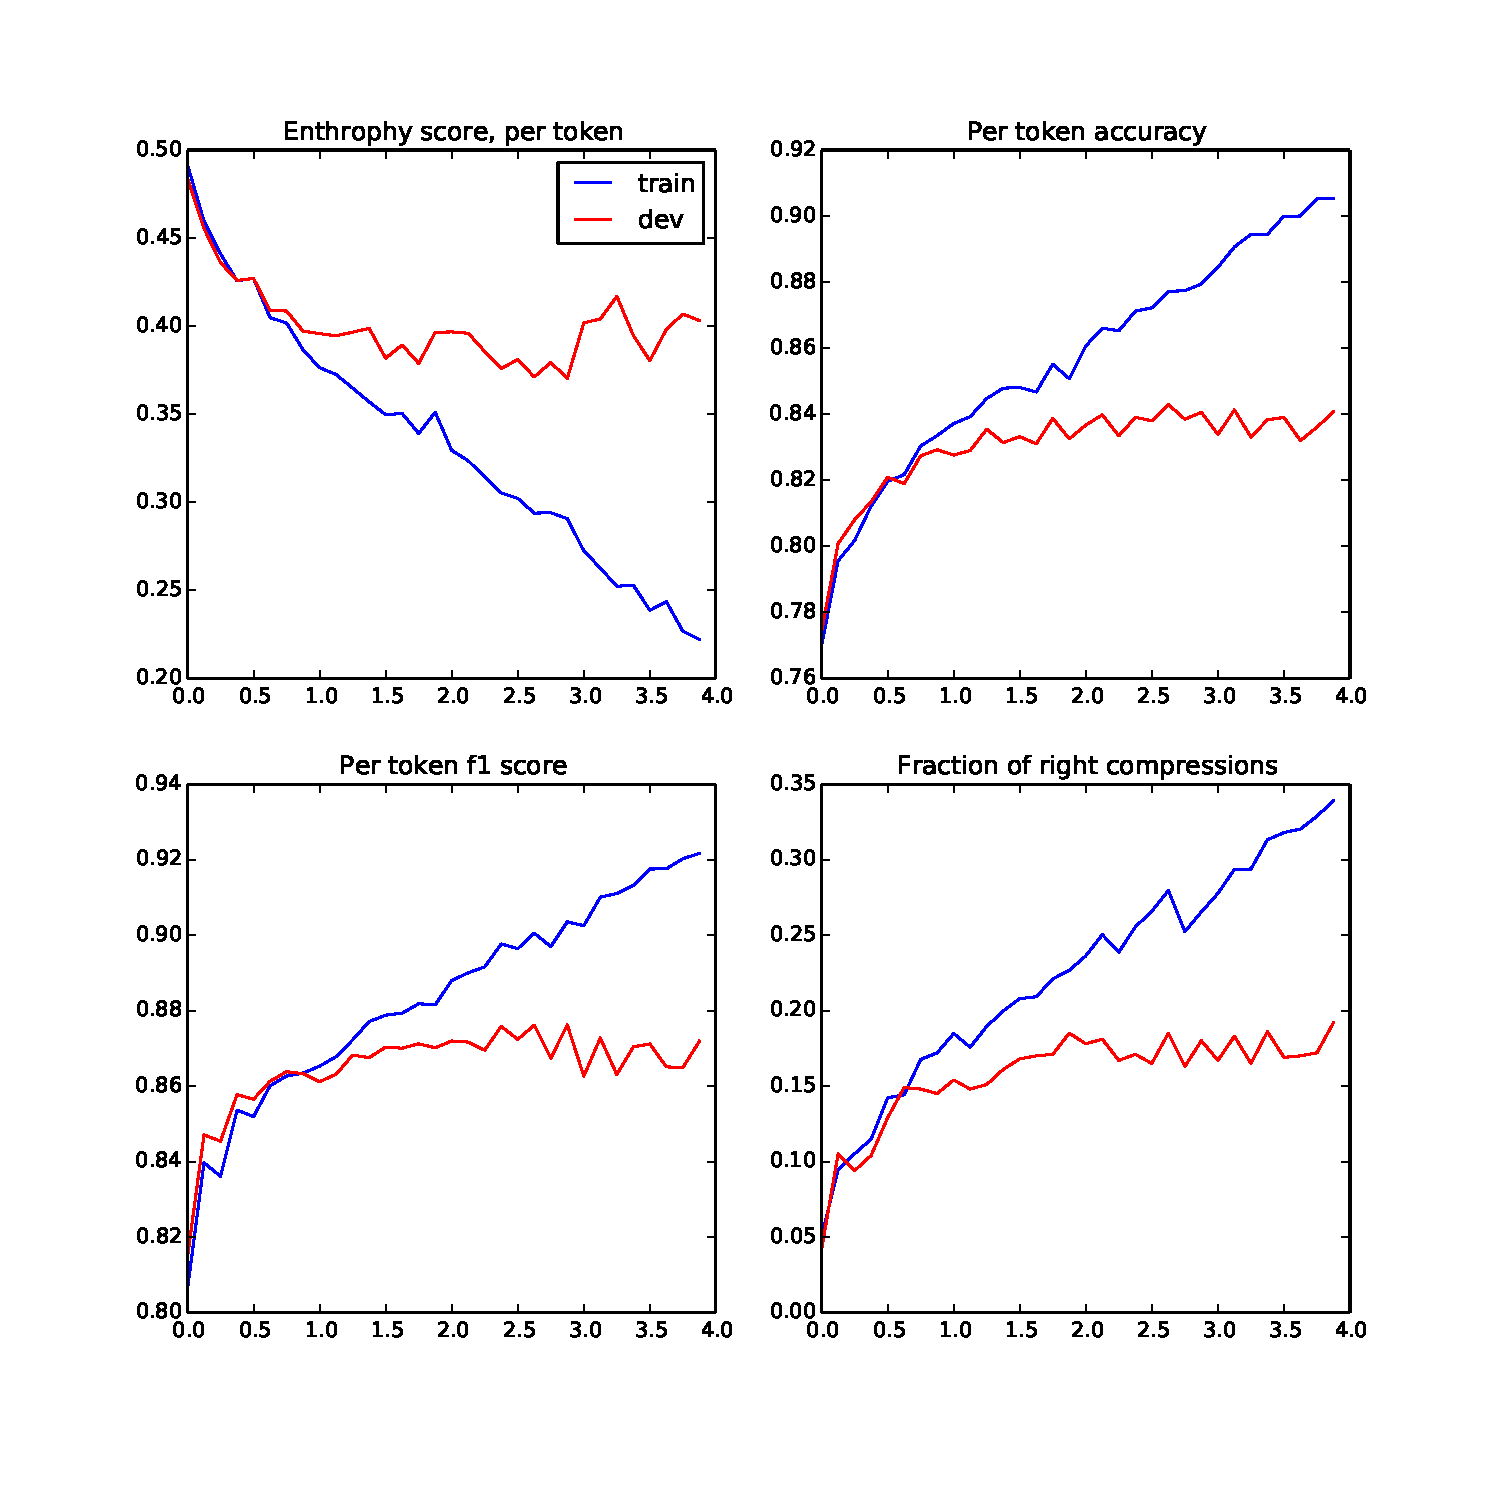
\includegraphics[width=\columnwidth]{learning_curves}
	\caption{The learning curves on train and dev sets}%
	\label{fig:lcur}%
\end{figure}


\begin{figure}[t]%
	\centering
	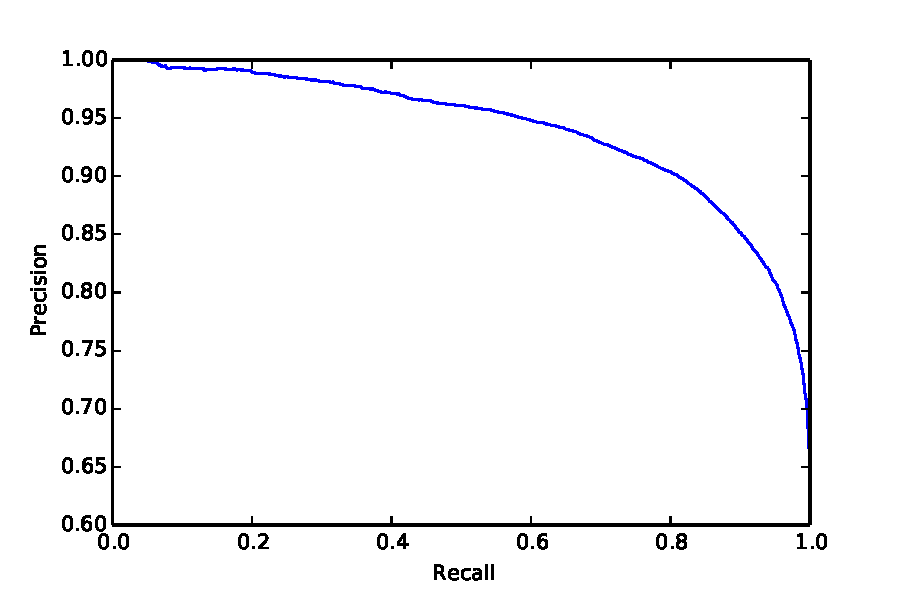
\includegraphics[width=\columnwidth]{precision_recal_curve}
	\caption{The Precision/Recall curve}%
	\label{fig:pr}%
\end{figure}

The table with compression examples can be found in \cref{table:gc} for good compression and \cref{table:b} for bad compression.

\begin{table}
\centering
\caption{Good compression}
\label{table:gc}
\csvreader[tabular=p{150pt}p{100pt}p{100pt},
    table head=\toprule Starting sentence & Reference  &  Predicted \\\midrule,
    table foot=\bottomrule,
    filter={\value{csvrow}<6}
]%
{good_compressions.csv}{Phrase=\Phrase,True=\True, Predicted=\Predicted}%
{\Phrase & \True & \Predicted \\\midrule}%
\end{table}


\begin{table}
\centering
\caption{Bad compression}
\label{table:b}
\csvreader[tabular=p{150pt}p{100pt}p{100pt},
    table head=\toprule Starting sentence & Reference  &  Predicted \\\midrule,
    table foot=\bottomrule,
    filter={\value{csvrow}<6}
]%
{bad_compressions.csv}{Phrase=\Phrase,True=\True, Predicted=\Predicted}%
{\Phrase & \True & \Predicted \\\midrule}%
\end{table}


\section {Conclusion}
In this project I implement an neural network solution to deletion-based sentence compression. Resulting network show good results on phrases with one subject and predicate. But not very good at phrases without subject, as well as complex phrases with 2 or more subjects.

 


\end{document}